\section {GLM}
The first matrix we get from convolution has five columns, which correspond to a column of ones and 4 cond.txt files in our dataset, respectively. After we get the convolution matrix, we use it as our design matrix to run the generalized linear regression on the image data. The dimension of our data is (64, 64, 34, 240), so, first we reshape our data into 2 dimensional array, which has the shape of (64*64*34, 240); the first dimension corresponds to 3-dimensional voxel indices and the second dimension corresponds to the time slice. Then we pass our design matrix into the glm function to calculate the related beta hats. Thus, there are in total 139624 beta hats that we get from the regression correspond to the first three dimensions of our image data. For example, the first beta hat contains the information about the voxel (0,0,0). Then we turn the beta hats back into 4-dimensional shape and run the diagnostic functions on the 4-d beta hats. Based on the predictors, we can calculate the fitted values and then the residuals. We use the MRSS of the first three dimensions as a measurement of our regression; in general, a smaller MRSS indicates a better performance of the regression model. 

\section {Smoothing} 
After we tried with the normal convolution matrix, we also generated high resolution convolution matrix and used it for linear regression. It turned out that the MRSS is just reduced by a little bit. Then we write a smoothing function to implement the multidimensional Gaussian filter on our data. We repeat the same procedures as what we have done in normal convolution on the smoothed data and the MRSS are reduced sharply. Therefore, we concluded that the smoothing method is a good pre-processing when we do the linear regression. 

\section {Hypothesis testing}
From linear regression, we can get t-statistics for different conditions(task on/off, gain, loss, distance).For each condition, we will have a 3D t-statistics matrix. For visualization, we first added mask based the mean voxel and the histogram. We set a boolean mask which takes larger than 375. Also we used smooth function and better color txt to generate a better image. Then we plotted the t statistics map for gain/loss. 
\begin{figure}[H] 
\centering 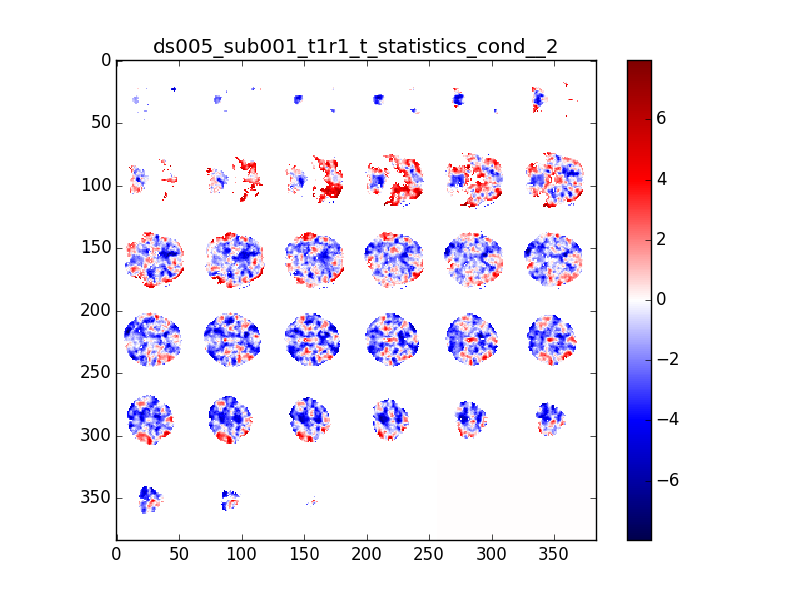
\includegraphics[scale=0.5]{../fig/t_test/ds005_sub001_t1r1_t-test_cond2.png}	 
\caption{T Statistics for Gain Subject 1 Run 1}
\end{figure} 
\begin{figure}[H] 
\centering 
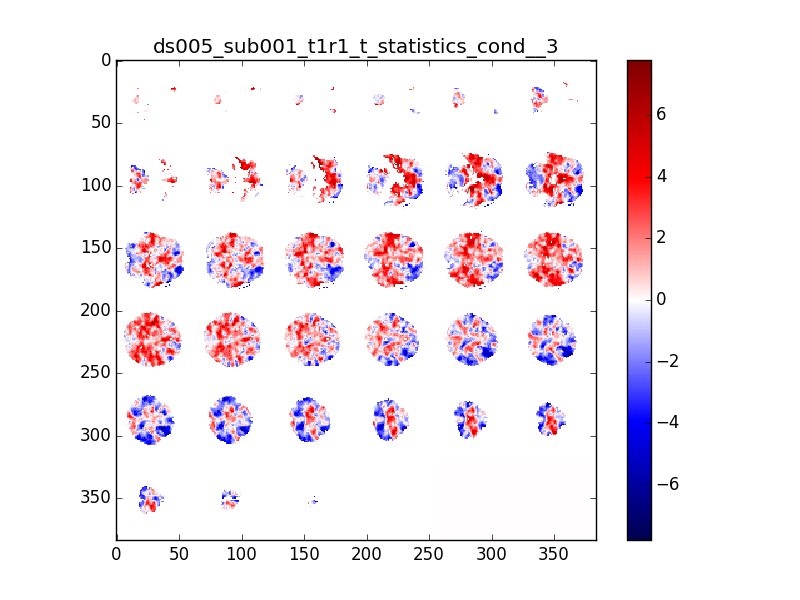
\includegraphics[scale=0.5]{../fig/t_test/ds005_sub001_t1r1_t-test_cond3.png} 
\caption{T Statistics for Loss Subject 1 Run 1}
\end{figure}
\begin{figure}[H] 
\centering 
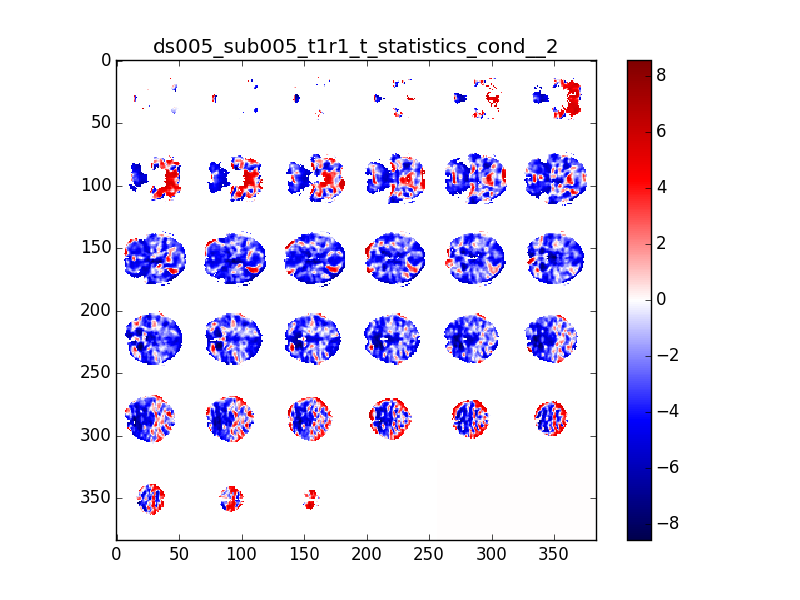
\includegraphics[scale=0.5]{../fig/t_test/ds005_sub005_t1r1_t-test_cond2.png}	 
\caption{T Statistics for Gain Subject 5 Run 1}
\end{figure} 
\begin{figure}[H] 
\centering 
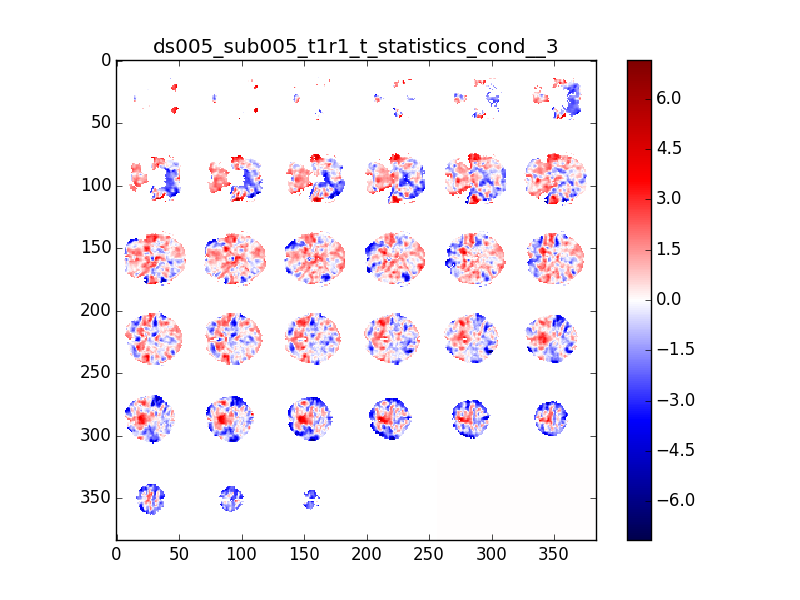
\includegraphics[scale=0.5]{../fig/t_test/ds005_sub005_t1r1_t-test_cond3.png} 
\caption{T Statistics for Loss Subject 5 Run 1}
\end{figure}  
\noindent
The larger the t-statistics, the more significant. Thus the red spots represents the activated voxels for gain and loss. For subject 1, gain has more activated voxels. However, for subject 5, loss has more activated voxels.

